\section{Missing mass resolution\label{sec-mmresol}}
The missing mass resolution $\sigma_{M_X}$ of the $^3$He($K^-,n$) reaction is expressed as,
\begin{eqnarray}
\sigma_{M_X}=c\times\sqrt{\left(\frac{\partial M_X}{\partial p_{beam}}\right)^2(\sigma_p^{beam})^2+\left(\frac{\partial M_X}{\partial p_{neutron}}\right)^2(\sigma_p^{neutron})^2},
\end{eqnarray}
where $\sigma_p^{beam}$ and $\sigma_p^{neutron}$ are the momentum resolutions of the kaon beam and the forward-going neutron, respectively. The contribution of the reaction-angle resolution is not considered since it is negligibly small ($<$7 mrad). The momentum resolution of the kaon beam is 2.0 $\pm$ 0.5 MeV/$c$ as discussed in Sec. \ref{sec-beammom} and that of the neutron is discussed in Sec. \ref{sec-ncres}. The missing mass resolution at the reaction angle of 0 degree with the beam momentum of 1 GeV/$c$ is shown in Fig. \ref{fig-mmresol}. The resolution satisfied our experimental requirement of $\sim$10 MeV/$c^2$ resolution at the region of interest.

\begin{figure}[]
\begin{center}
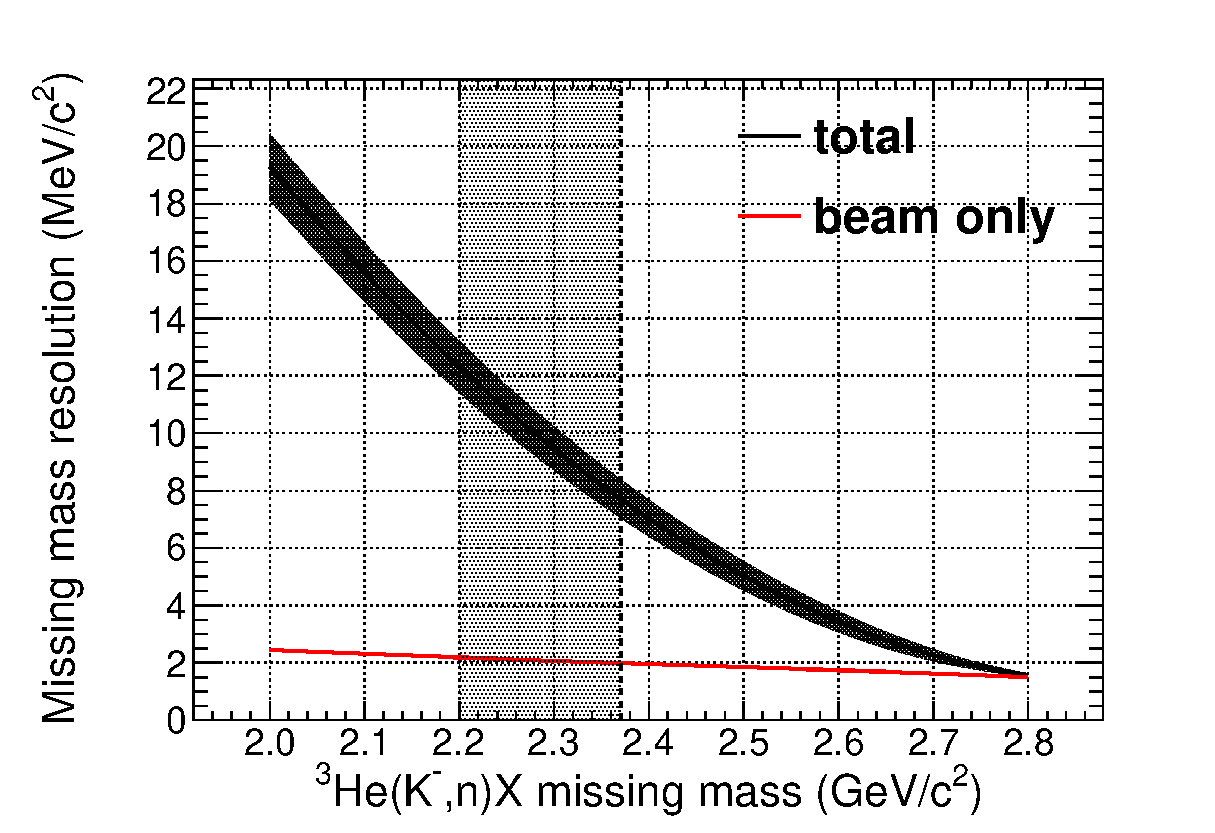
\includegraphics[width=12cm]{./fig/mm-resol.eps}
\caption[Missing mass resolution of the $^3$He($K^-,n$) reaction.]{Missing mass resolution of the $^3$He($K^-,n$) reaction. The vertical dotted line and the hatched area represent the $K^-pp$ binding threshold and the region of interest, respectively.}
\label{fig-mmresol}
\end{center}
\end{figure}  

\section{Precision of the missing mass scale\label{sec-scale}}
To determine absolute missing mass scale of the $^3$He($K^-,n$) reaction, the beam momentum was calibrated at first by the forward-proton spectrometer as described in Sec. \ref{sec-beammom}. Then the neutron momentum was evaluated by reconstructing the invariant masses of $\Sigma^\pm\to n\pi^\pm$ decays. In addition, we checked the the residual-nucleus peaks in the missing masses of $^3$He($K^-,nK^0_s)d$, $^3$He($K^-,npK^-)p$, and $^3$He($K^-,np\pi^+\pi^-)n$ reactions. In these studies, the neutron and the charged particles were measured with the NC and the CDS, respectively.

\subsection{Reconstruction of the $\Sigma$s and the residual nucleus}
\subsubsection{$\Sigma$ reconstruction}
The $\Sigma^\pm$ hyperons are mainly produced by quasi-free processes of $K^-+p\to\pi^\mp\Sigma^\pm$. The forward-going $\Sigma$s were reconstructed by detecting $\Sigma^\pm \to \pi^\pm n$ decays, where the pion and the neutron were measured with the CDS and the NC, respectively. The reconstructed $\pi^\pm n$ invariant mass distributions are shown in Fig. \ref{fig-sigmaraw}, where $\Sigma^\pm$ peaks are clearly identified. Since two pions are emitted from the $K^-+p\to\pi^\mp\Sigma^\pm$ reactions, the signal-to-noise ratios of the $\Sigma^\pm$ would increase by requiring an additional pion. Red histograms in Fig. \ref{fig-sigmaraw} are the $n\pi^\pm$ invariant mass spectra with the two pion selection, and we evaluated the peak position of the $\Sigma^\pm$ using the histograms. Since the neutron momentum from $\Sigma$ decay has wide distribution with rather large statistics, the peak positions were evaluated for five $^3$He($K^-,n)X$ missing-mass ranges; (2.27,2.37), (2.37,2.47), (2.47,2.57), (2.57,2.67), and (2.67,2.77) GeV/$c^2$.

\begin{figure}[]
\begin{center}
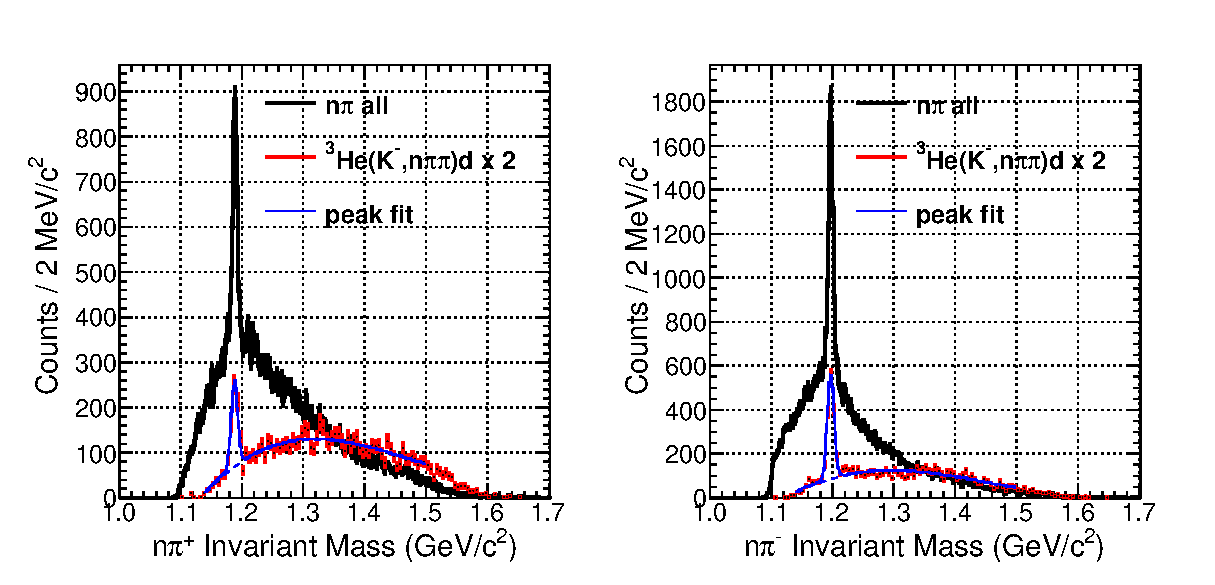
\includegraphics[width=\columnwidth]{./fig/sigma-raw.eps}
\caption[Invariant mass distributions of $n\pi^+$ and $n\pi^-$.]{Invariant mass distributions of (left) $n\pi^+$ and (right) $n\pi^-$. The red histograms require $n\pi^+\pi^-$ detection and the $^3$He($K^-,n\pi\pi)X$ missing mass to be consistent with a deuteron. They are scaled by factor two.}
\label{fig-sigmaraw}
\end{center}
\end{figure}  

\subsubsection{Spectator deuteron in quasi-free $K^0_s$ production}
In the quasi-free reactions on a proton in the $^3$He target, the spectator is a deuteron or a pair of a neutron and a proton. Especially in the quasi-free $K^0_s$ production, $K^-+p\to K^0_s+n$, we can easily identify the spectator by using the $K^0_s\to \pi^+\pi^-$ decay and the forward-going neutron detected with the CDS and the NC, respectively. As shown in Fig. \ref{fig-k0missd}(left), clear strength around the deuteron mass can be seen in the $^3$He($K^-,nK^0_s)X$ missing mass. By requesting the small missing-momentum, we can enhance deuteron spectator events from the contaminations, where a neutron and a proton are unbound. Figure \ref{fig-k0missd}(right) is the $^3$He($K^-,nK^0_s)X$ missing-mass distribution with the missing momentum less than 150 MeV/$c$, and the peak position corresponding to deuteron mass was evaluated using the histogram. 
\begin{figure}[]
\begin{center}
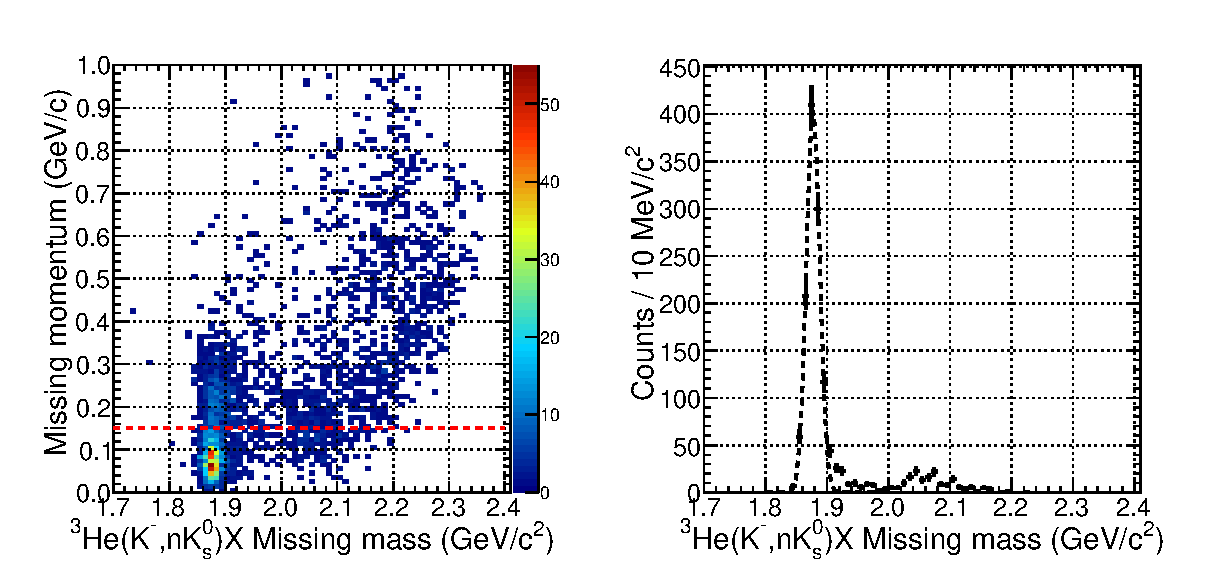
\includegraphics[width=\columnwidth]{./fig/k0-missd.eps}
\caption[$^3$He($K^-,nK^0_s)X$ event distribution.]{(left) Correlation between the missing momentum and the missing mass in the $^3$He($K^-,nK^0_s)X$ reaction. (right) The missing-mass distribution with the missing momentum of less than 150 MeV/$c$, which is indicated as a red-dotted line in the left figure. The spectator deuteron peak was fitted with a Gaussian.}
\label{fig-k0missd}
\end{center}
\end{figure}  

\subsubsection{Spectator proton and neutron in multi-nucleon absorption( or two-step) processes}
We measured multi-nucleon absorption (or two-step) processes whose final-state particles were a proton and charged mesons detected with the CDS and neutron detected with the NC. Among them, the missing mass distribution of the $^3$He($K^-,npK^-)X$ and $^3$He($K^-,np\pi^+\pi^-)X$ reactions are shown in Fig. \ref{fig-pknmissp}(left) and \ref{fig-pknmissn}(left), respectively. The spectator proton and neutron are clearly seen in the figures, and we evaluated the missing mass scale using the peaks of spectators. Fig. \ref{fig-pknmissp}(right) and \ref{fig-pknmissn}(right) show the $^3$He($K^-,n)X$ missing mass distributions for those events. 
\begin{figure}[]
\begin{center}
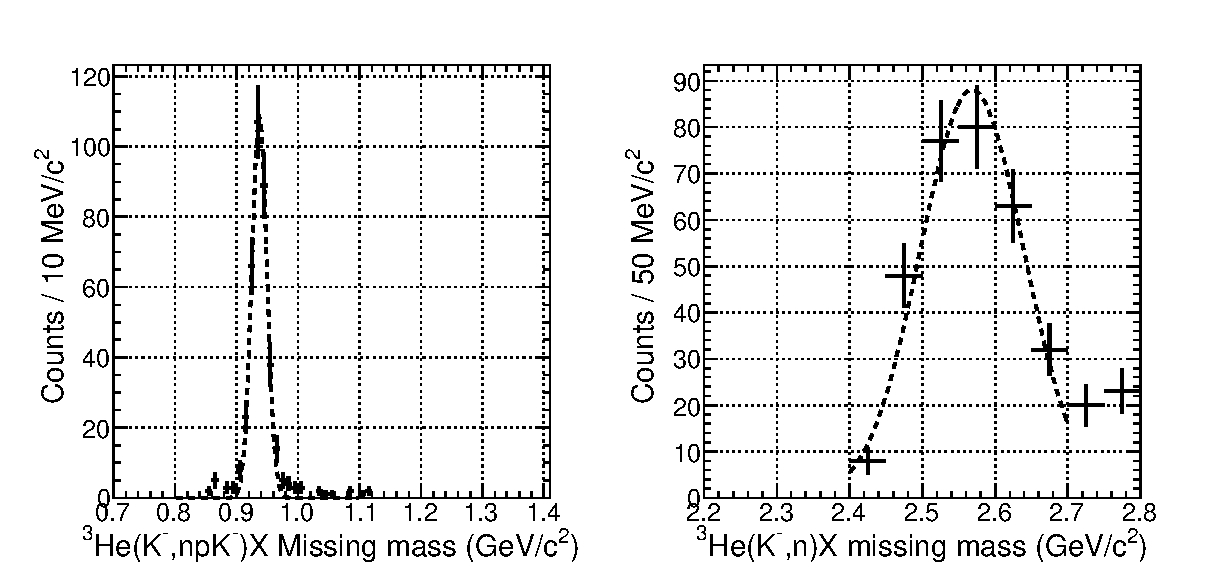
\includegraphics[width=\columnwidth]{./fig/pkn-missp.eps}
\caption[$^3$He($K^-,npK^-)X$ event distribution.]{(left) $^3$He($K^-,npK^-)X$ missing-mass distribution with the missing momentum of less than 150 MeV/$c$. The spectator proton peak was fitted with a Gaussian. (right) $^3$He($K^-,n)X$ missing-mass distribution corresponding to the left histogram. The distribution was roughly parametrized by a Gaussian.}
\label{fig-pknmissp}
\end{center}
\end{figure}  

\begin{figure}[]
\begin{center}
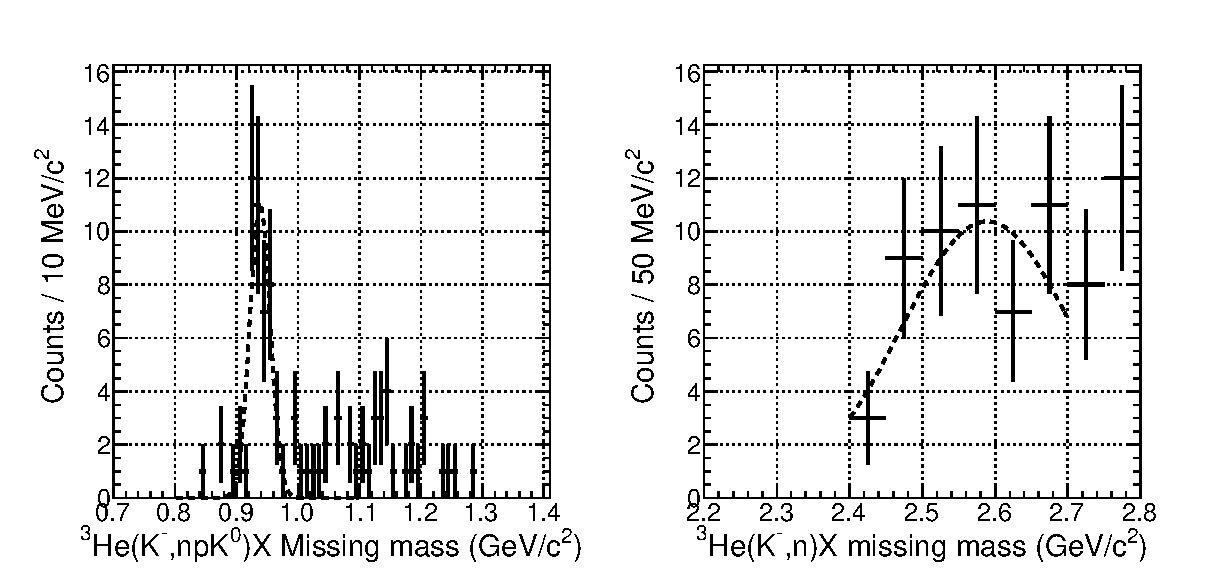
\includegraphics[width=\columnwidth]{./fig/pkn-missn.eps}
\caption[$^3$He($K^-,np\pi^+\pi^-)X$  event distribution.]{(left) $^3$He($K^-,np\pi^+\pi^-)X$ missing-mass distribution. The spectator neutron peak was fitted with a Gaussian. (right) $^3$He($K^-,n)X$ missing-mass distribution corresponding to the left histogram. The distribution was roughly parametrized by a Gaussian.}
\label{fig-pknmissn}
\end{center}
\end{figure}  

\subsection{Precision of the absolute missing mass scale}
Centroids of above five peaks were obtained in the spectral fitting, and $^3$He($K^-,n)X$ missing-mass dependences of their deviations from the PDG masses are shown in Fig. \ref{fig-enescale}. All of the centroids are consistent with the PDG values within 3 MeV/$c^2$. Therefore, the validity of the absolute missing-mass scale was confirmed with the systematic error of 3 MeV/$c^2$.
\begin{figure}[]
\begin{center}
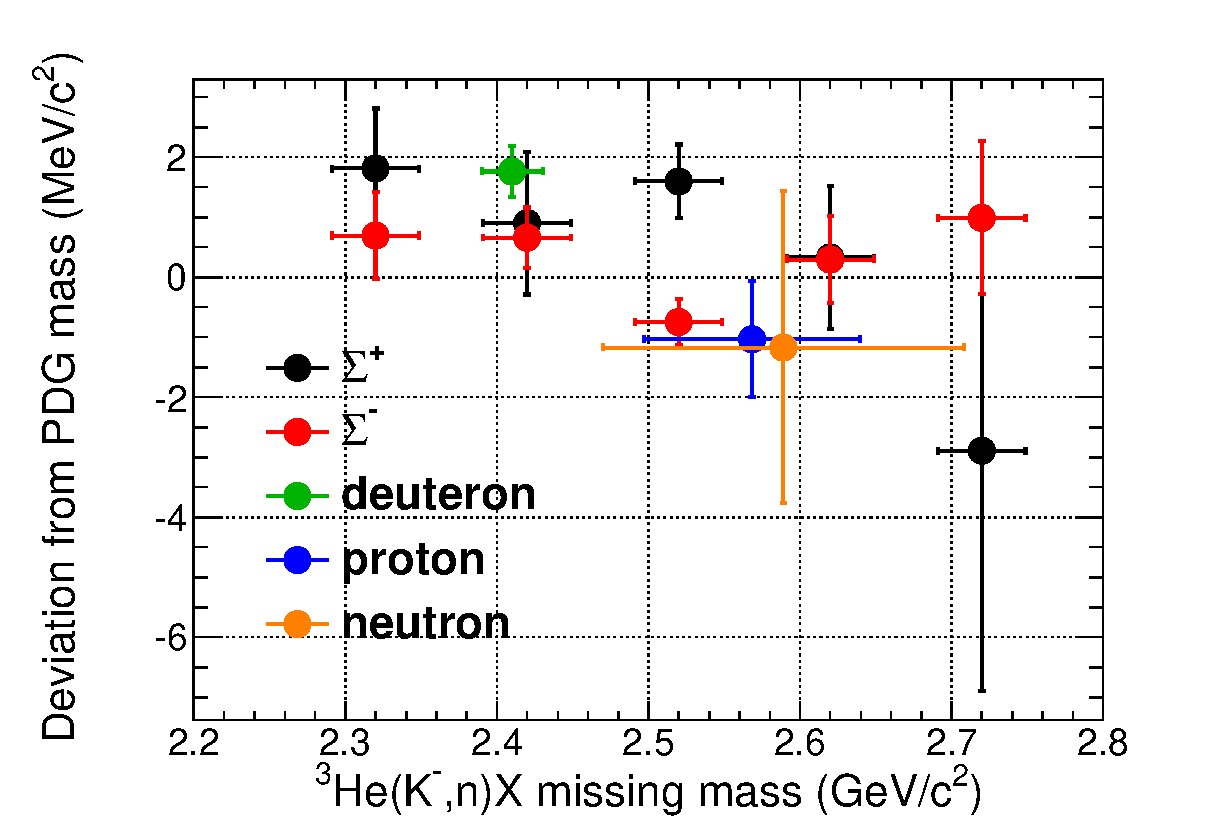
\includegraphics[width=12cm]{./fig/enescale.eps}
\caption[Summary of the evaluation of the mass-scale precision.]{$^3$He($K^-,n)X$ missing-mass dependences of the mass deviations between the reconstructed values and the PDG ones for each particle. The signs for the $\Sigma$s are inverted. }
\label{fig-enescale}
\end{center}
\end{figure}  

\subsubsection{}